\documentclass[12pt,a4paper]{article}

% Essential packages
\usepackage[utf8]{inputenc}
\usepackage[T1]{fontenc}
\usepackage{lmodern}
\usepackage[english]{babel}
\usepackage{amsmath,amsfonts,amssymb}
\usepackage{graphicx}
\usepackage[margin=2.5cm]{geometry}
\usepackage{setspace}
\usepackage{fancyhdr}
\usepackage{titlesec}
\usepackage{caption}
\usepackage{subcaption}
\usepackage{booktabs}
\usepackage{array}
\usepackage{multirow}
\usepackage{longtable}
\usepackage{adjustbox}
\usepackage{siunitx}
\usepackage{float}
\usepackage[hidelinks]{hyperref}
\usepackage{xcolor}
\usepackage{colortbl}

% Page setup
\onehalfspacing
\pagestyle{fancy}
\fancyhf{}
\fancyhead[L]{K-Epsilon CFD Analysis}
\fancyhead[R]{\thepage}
\renewcommand{\headrulewidth}{0.4pt}

% Title formatting
\titleformat{\section}{\large\bfseries}{\thesection}{1em}{}
\titleformat{\subsection}{\normalsize\bfseries}{\thesubsection}{1em}{}
\titleformat{\subsubsection}{\normalsize\bfseries}{\thesubsubsection}{1em}{}

% Table setup
\renewcommand{\arraystretch}{1.2}
\setlength{\tabcolsep}{6pt}

% Custom colors for tables (matching original)
\definecolor{lightblue}{RGB}{207,226,243}
\definecolor{mediumblue}{RGB}{159,197,232}
\definecolor{darkblue}{RGB}{61,133,198}
\definecolor{navyblue}{RGB}{11,83,148}
\definecolor{lightgreen}{RGB}{0,255,0}
\definecolor{red}{RGB}{255,0,0}

\begin{document}

% Title Page
\begin{titlepage}
\centering
\vspace*{2cm}
{\LARGE\bfseries Analysis of K-Epsilon Computational Model in ANSYS:\\[0.5cm] 
Impact of Mesh Density and Iterations on Turbulent Flow Prediction Accuracy for Complex Geometries}\\[2cm]

{\large A Research Investigation into Computational Fluid Dynamics}\\[1.5cm]

{\large Submitted by: [Student Name]}\\[0.5cm]
{\large Student ID: [Student ID]}\\[0.5cm]
{\large Course: [Course Code]}\\[0.5cm]
{\large Institution: [University Name]}\\[1.5cm]

{\large Date: \today}\\[2cm]

\vfill
\end{titlepage}

% Table of Contents
\newpage
\tableofcontents
\newpage

% List of Figures
\listoffigures
\newpage

% List of Tables
\listoftables
\newpage

\section{Introduction}

\subsection{Background}

Ib fluid drag formula:

The IB supplies a simplified equation and theory behind fluid drags on objects, F rv d = 6πηr, which assumes all objects are round, and flow is laminar, this creates allot of limitations that the simulations should eliminate

CFD: 

Computational fluid dynamics simulations are computer simulations of fluid flow. They are used to analyse and solve problems in fluid flow, heat transfer and similar activities. They rely on heavy software and computational power to simulate difficult situations which are hard to simulate experimentally. 

It involves a lot of physics equations, especially the Navier stokes and the Reynolds equations, to calculate pressure velocity, temperature, and density of a fluid over time in different situations, from which drag can also be calculated. It is very important in various industries: Aerodynamics (e.g., aircraft design, drag reduction), Automotive engineering (e.g., optimizing car shapes for fuel efficiency), Energy (e.g., modeling wind turbines, heat exchangers), Medicine (e.g., studying blood flow in arteries).

K-epsilon:

CFD simulations run on different models, the model that i am choosing is the K-epsilon model, it is a very popular model used in a lot of amateur and beginner simulations, which don't require a niche model.

The k-episode model was developed by Launder and Spalding in 1974 to improve on older models like the mixing length model. It offers a more general and practical approach to modeling complex turbulence and flows. It majorly uses two equations, one for turbulent kinetic energy and one for dissipation rates.

This model is often used in simulating airflows in HVAC systems and combustion in engines, analysing drag and lift on vehicles, Modeling the travel of particles like pollutant through water and the atmosphere and studying flow in pipes, channels and bridges

The model predicts the mean flow characteristics of flows, by solving the two equations, it is assuming isotropic turbulence, which means the turbulent viscosity is equal across every direction, this makes it very suitable for many engineering applications. Though It does struggle with the investigated complex geometries.

why is the model good?

Because the model only uses two equations to calculate the simulation its simplisity matches its power. It is great for a wide range of reynolds number of flows, so it is perfect for simulating turbulence. The model shows to converge correctly, in simulation converging is referred to when multible sennerios and calculations give the same answer which means the answer is likely to be very precise. And as the model has been used since 1974 it has had decates of testing impovements and validation

There are better models out ther now as the k-omega sst, which can handle bigger pressure drops accros the simulation, but that model is even more power hungry and expensive to run. The k-epsilon model is not very good at calculating swirls and flows including strong separation in the fluid.

Why is Asyns good?

I am using a student version of the ansys software which is running all the simulations, asyns is such a good choice, because it has incredible horizon of simulation choices, it offers more then just fluid dynamics, but it can also simulate things like heat transfer and electromagnetic fields. This makes it very appealing for engineers. 

Over 17.000 companies use asyns, including racign and rocket teams liek nasa and redbull racing.

Mesh density?

This investigation is investigating the affect of mesh density on time, now why does mesh density actually matter?

\begin{figure}[H]
    \centering
    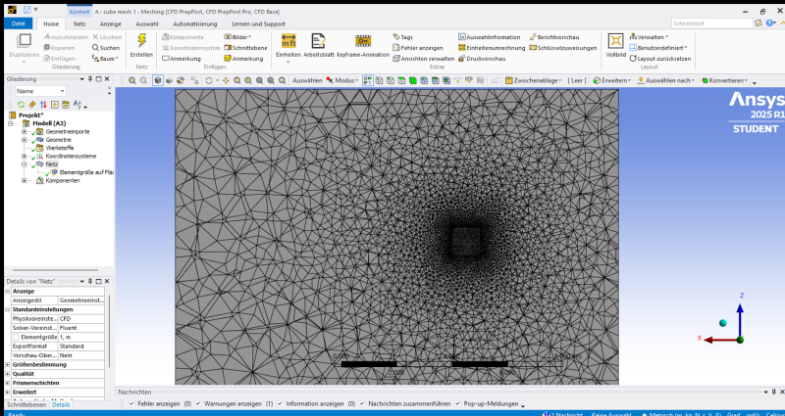
\includegraphics[width=0.8\textwidth]{image9.png}
    \caption{Mesh visualization of a complex geometry showing triangular elements with varying density}
    \label{fig:mesh_example}
\end{figure}

above is a image of the mesh of one of the complex objects simulated in the experiment. Mesh density can metaphorically be refferet to as resolution, imagine every one of the triangles above is a pixel on your screen, the more triangles your have per area like in the middle right of the image the better the resolution. A simulation calculates the physical behavior of every triangle. In real life we have incredibly small particles which all follow the laws of physics, and the closer we get to the size of the particle the more accurate does our simulation follow real life, but that also means more calculations need to be doen, and possible more time will be allocated to the simulation.

Calculations are only done inside the grey area, i have made sure that there is enough volume for the simulation to take into account everything which is relevant. which means the simulation is ignoring everything else, which could happen outside of the blocks volume-. This volume is constant throughout the experiment though.

Why does the amount of itterations matter?

In simulation iterations refers to the amount of scenarios,The scenarios refer to testing different temperatures, velocities and pressure in different places. for which all calculations are done. Like in statistics the bigger the sample size the smaller the random error. And the standart diviation of all findings will get smaller aswell. 

\begin{figure}[H]
    \centering
    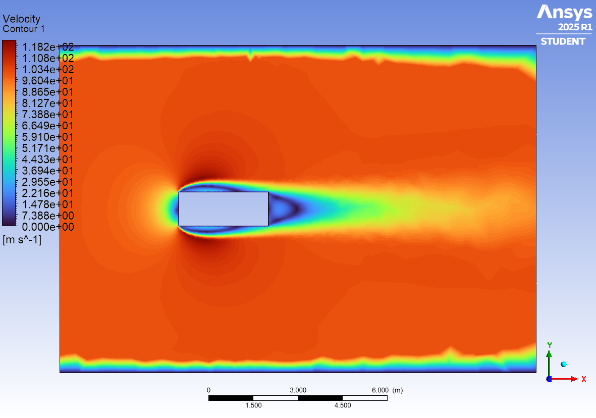
\includegraphics[width=0.8\textwidth]{image8.png}
    \caption{Simulated drag results versus iteration number showing convergence behavior}
    \label{fig:convergence}
\end{figure}

In the graph above, i have displayed the simulated drag results y against the amound of iterations x, visible is that after 20 itterations the simulated drag is not really changing this is reffered to as converging. But before testing all scenarios one will never knwo if the values change, so there is a incentive to have almost infinite amount of itterations. Having infinite amount of itterations is bad though, because for every itteration a complete calculation of all physics behaviours needs to be done. so more itterations mean more time.

Residuals?

One of the constant of this investigation are residuals, residuals govern how far the simulation will run intill the values converge. they do this by reflecting the imbalance in the conservation laws, mass enegy…, in the navier stokes equations, low residulas means more pressice measurements and high residuals mean low precition. The residuals therefore basically define too how many significant figures the calculation are hold truthfully, in the experiment i have defined all residuals to 5 digit accuracy, which in return means 5 significant figures for my result, i have chosen 5 digits and not 6 digits or lower, because when running tests at 6 digit accuracy, the test did not converge even after 1000 itteration and as seen in the graph above for the iterations this means the simulations could have taken even longer and return no relativly more valueble insights. 

All simulations in this experiment are run to either all residuals converge, which means the number calculated is the number the computer thinks is most accurate, or to 1000 itteration, because that can indicate that there is a error with the geometry or the mesh of the simulation and the simulations is likely faulted, or and can not get more accurate.

Is my experiment accurate?
The goal of my experiment is to find out how much we acctualy need to simulate things untill they become accurate enough. In real life we often dont simulate cubes and other simpler shapes but these are still more complex shapes than the sphere we assume in ib, but all bodies and shapes in some way or the other will kind of reflect or can be build up from the chapes that i am simulating, for example a plane can be simplified to one longe cylinder with a half sphere at the front and wide water droplets as wings. Now firms like nasa which relly on some base of simulations for there space flight programm have acces to computationally way stronger hardware compared to me, so the acctual time they are invest is far lower then mine, but the waisted time from letting simulations run for to long, relative to mine is still the same.

\subsection{Aims and Objectives}

In the k-epsilon computational model in ansys how does the time invested into calculation heavy mesh and iteration affect the accuracy of prediction of turbulent flow characteristic fpr complex geometries?

In this experiment i will try and compare diffrent simulation set ups, so diffrent mesh densities and amounts of itterations, against experimental values of fluid drag widely considered true. Through this i try to evalute how accurate simulations can get or should get in reference to the values obtained in the wing tunnel.

Now it might seem like i have two depend variables and two independent, but actually i am measuring the wasted time from simulating to no accuracy benefit created by the variables instead, i need both of them to understand what is actually waisting the time. I am measuring the time waisted, because our computers are consuming powers in watt, which means the longer the simulation takes the more power is consumed, assuming the time is wasted because the simulation is not getting more accurate as i stated this would mean the power is wasted aswell and in our day and age wasting power goes against allot of humanities goals. This ofcourse requires the assumption that all computtions did require the same power.

\section{Literature Review}

\subsection{The Physics of Fluid Flow}

Now in ib we assume fully laminar flow, for engeering this assumption might not result in pleasing result. Because laminar flow only happens in very viscous fluids or in very stream line bodies. In refrence to fluid drag this means only drag in the form of skin friction will get calculated.

Turbulent flow means the the fluid creates chaotic and swirling eddies, for egneniers turbulent flow is often very real. It applies at high velocities or when the geometry are more complex and the viscosity of fluids is low liek air. In reference to fluid drag turbulence introduces new kinds of drag like pressure drag, this drag is created when the eddies create flow separation allongsaide the object, so turbulent calculations need to consider the stream lines of objects, referred to as cd, the ib formula does not consider this at all and only considers drag created directly on the front face of the objects. 

Turbulant flow does not definitely mean that the drag is higher thoug, golf balls for example use there very unsteamline shape to benefit from the turbulent flow in a way that the actual drag is reduced.

\subsection{Computational Fluid Dynamics (CFD)}

As i said before the k epsilon model uses two equations to calculate the physical behaviour of particles.
the navier stokes equation: 
\begin{align}
\text{Continuity: } \nabla \cdot \vec{u} &= 0\\
\text{Momentum: } \rho\left(\frac{\partial \vec{u}}{\partial t} + \vec{u} \cdot \nabla \vec{u}\right) &= -\nabla p + \mu \nabla^2 \vec{u} + \vec{f}
\end{align}

Is what physicist would use to do such calculations, and in ib our fluid drag formula uses a simplification of this formula, because the equations are nonlinear and interdependent it is very difficult to calculate specific behaviour especially when turbulent flow is introduced, for the same reason the k-epsilon model actually also uses a simplicication of this equation aswell.

Instead the model uses the reynolds average stokes equations,
\begin{equation}
\rho\left(\frac{\partial \overline{u_i}}{\partial t} + \overline{u_j}\frac{\partial \overline{u_i}}{\partial x_j}\right) = -\frac{\partial \overline{p}}{\partial x_i} + \mu\frac{\partial^2 \overline{u_i}}{\partial x_j^2} - \frac{\partial \rho\overline{u_i' u_j'}}{\partial x_j}
\end{equation}

This equation introduces turbulence and averages the stokes equations making it possible to calculate the behavoir of particles, interesting is that this equation is viewing mean and fluctuating variables at the same time, this means that from the mesh picture the surrounding triangles also affect the individuel triangle, very muhc like how all particle affect each other.

\section{Methodology}

\subsection{Experimental Approach}

The value i am finding through the simulation, will be compared to a highly extensive researched database.

\subsection{Computational Simulation}

Using Ansys, a computer simulation software, the drag forces experienced by the objects will be simulated. i will be changin two variables to see the affect on the accuracy of the simulation outcome and how long the simulation needs to finish, Mesh density and the amount of iterations, because i predicted them to have the biggest impact on the time taken for the simulations to finish. I will use this formula $F_d = \frac{c_d \rho u^2 A}{2}$ to compare my simulated drags forces, to forces i calculated using the Cd aquired experimentaly. 

To be sure that all other variables are sensible i have set them as follows. The air speed at which the drag will be simulated will be 100ms$^{-1}$, this is because drag will increase significantly at close to mock numbers due to the increased pressure of the schock cone, but the drag at low velocity is very small and sometimes insignificant, exactly what value is chosen is not important, as long it is constant in the comparison calculations. 

I have set the air density used in the simulation to 1.225 kgm$^{-3}$ which is the standart setting in Ansys, but is also standart air pressure, this variable could also be changed, it just needs to be constant in the comparison though.

 I have set the area of the geometries facing the air stream to be equal to 1m$^2$; although also this value is arbitrary, i think using 1m$^2$ will be helpful in the future, when making predictions on geometries which are bigger, because than the ratio is just the bigger size divider by one. 

I will be testing different mesh densities, which i calculate by the number of mesh elements divided by the volume of the perimeter in which the simulation is taking place, as that volume is also constant across all simulations i will refer to the mesh only by the amount of elements.

I am not changing the total amounts of mesh directly, instead i am changing the size of the elements close to the object. This is common use and is useful, because i would not expect allot of physics behaviour far away from the geometrie for which i want to calculate the drag, 

\begin{figure}[H]
    \centering
    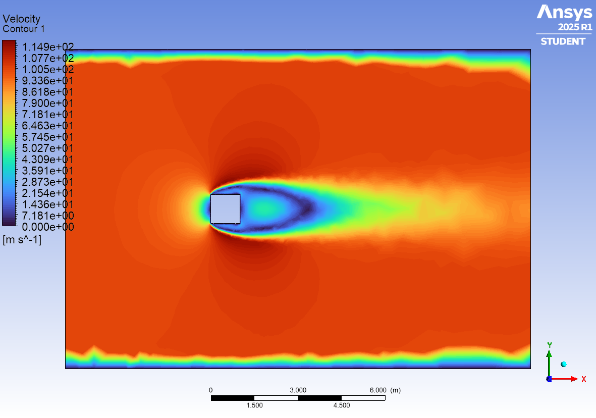
\includegraphics[width=0.8\textwidth]{image1.png}
    \caption{Flow visualization showing physics behavior primarily near the cube geometry}
    \label{fig:flow_viz}
\end{figure}

As seen above the flow is mostly just red further away from the cube, this indicated that there is no physics behaviour happing there. i have labelled the msot dense mesh 5 and the least dense mesh 1, from my hypothesis i would expect the 5 one to take the longest and have the most accurate results, although not significantly more accurate then say 3 or 4. 

The general mesh size of the simulation parameters is 1 m$^3$, this means that calculations are done for that 1 m$^3$ and the simulation assumes one particle has the size of 1 m$^2$ and it will calculate a mean physics behaviour for that whole area. I have set the most accurate mesh elements to be 0.05m$^3$ big directly next to the geometries, this is significantly smaller than both the general mesh size and the geometrie, so it should give accrued calculation results. Because if we go back to the screen analagie, it is only possible to show a elephant for example if the pixels are smaller than the elephant which i am trying to display, in this case the mesh element size is smaller then the geometry so it should be possible to simulate it.

\begin{table}[H]
\centering
\caption{Mesh configuration for cube geometry}
\label{tab:mesh_config}
\begin{tabular}{|c|c|c|c|c|c|}
\hline
\rowcolor{red!50}
\textbf{Mesh} & \textbf{1} & \textbf{2} & \textbf{3} & \textbf{4} & \textbf{5} \\
\hline
element size /m & 0.25 & 0.2 & 0.15 & 0.1 & 0.05 \\
\hline
number of elements & 52168 & 68605 & 97258 & 153590 & 341044 \\
\hline
\end{tabular}
\end{table}

In the last row i have writin the total amount of elements, this number is not significant, i can not change it directly i can only impact the element size, the number of elements is only what i can measure, i will get back to size, but because the element sizes are used equally across all geometries to get a more accurate comparison i wiil use the amount of elements which arent equal across all geometries later for comparison. This is because some geometries might take less time to simulate and be less accurate eventhough they have same mesh size, because they are smaller by themselves, remember i have to scale all objects to have a frontal area of one, but some objects are longer than others. For every mesh size i will run the simulation again, i will then write down the total number of iterations the simulations hade to do before converging, if the simulation never converged i have capped the maximum number of iterations at 1000, then i will take readings of the drag force at every 1/5 amount of all iterations, this should give me some kind of understanding, how the accuracy is changing over the run of the experiment.

\begin{table}[H]
\centering
\caption{Example of iteration documentation, for the mesh3 of the cube}
\label{tab:iteration_example}
\begin{tabular}{|c|c|c|c|}
\hline
\rowcolor{red!50}
\textbf{total Iterations} & \textbf{218} &  &  \\
\hline
\textbf{1/5 of total Iterations} & \textbf{2/5 of total Iterations} & \textbf{3/5 of total Iterations} & \textbf{4/5 of total Iterations} \\
\hline
44 & 87 & 131 & 174 \\
\hline
\end{tabular}
\end{table}
\section{Results and Discussion}

\subsection{Experimental Results}

\begin{figure}[H]
    \centering
    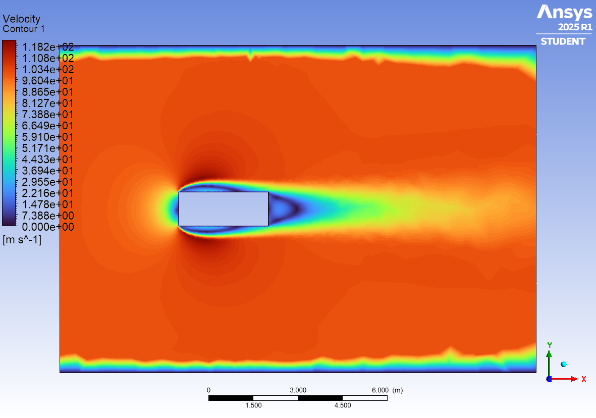
\includegraphics[width=0.8\textwidth]{image8.png}
    \caption{Simulation monitoring display during runtime}
    \label{fig:simulation_display}
\end{figure}

This is what i can view when the simulation is running, already from this one can see that nothing really changes allot in the run of the simulation. Not every graph looked as clean as this one for the cube.

\begin{table}[H]
\centering
\caption{Full data collected for the cube simulation}
\label{tab:cube_results}
\adjustbox{width=\textwidth}{
\begin{tabular}{|c|c|c|c|c|c|c|c|c|c|c|c|}
\hline
\textbf{Iteration} & \textbf{Expected /N} & \textbf{Mesh 1 /N} & \textbf{\% error} & \textbf{Mesh 2 /N} & \textbf{\% error} & \textbf{Mesh 3 /N} & \textbf{\% error} & \textbf{Mesh 4 /N} & \textbf{\% error} & \textbf{Mesh 5 /N} & \textbf{\% error} \\
\hline
1/5 of total & 6.43E+03 & 5.72E+03 & 11.01\% & 5.98E+03 & 6.96\% & 6.07E+03 & 5.67\% & 6.23E+03 & 3.19\% & 6.04E+03 & 6.04\% \\
\hline
2/5 of total & 6.43E+03 & 5.72E+03 & 11.04\% & 5.97E+03 & 7.15\% & 6.08E+03 & 5.47\% & 6.30E+03 & 2.08\% & 6.38E+03 & 0.84\% \\
\hline
3/5 of total & 6.43E+03 & 5.72E+03 & 11.01\% & 5.97E+03 & 7.20\% & 6.10E+03 & 5.22\% & 6.30E+03 & 2.02\% & 6.42E+03 & 0.18\% \\
\hline
4/5 of total & 6.43E+03 & 5.73E+03 & 10.97\% & 5.97E+03 & 7.19\% & 6.09E+03 & 5.26\% & 6.30E+03 & 2.00\% & 6.43E+03 & 0.07\% \\
\hline
5/5 of total & 6.43E+03 & 5.72E+03 & 10.99\% & 5.97E+03 & 7.17\% & 6.09E+03 & 5.29\% & 6.30E+03 & 2.01\% & 6.43E+03 & 0.06\% \\
\hline
\end{tabular}
}
\end{table}

This is the table of measurements which i have found for the cube, written down in under the meshes headings is the simulated drag force experienced by the cube, they are to 5 significant figures, but the data base only has 3 significant figures therefore i will only visually compare only the first 3, but use the unroundet numbers for the \% error.

now we can see that the simulation has found an incredible accurate force after the simulations finished so after all iterations, and with the highest mesh density, of 99.94\% i was not expecting this, remember the software is not interpreting forces from a databank, but it is calculating it purely from its understanding of the laws of physiks, also to be seen is that atleast until ⅗ of the total simulation the accuracy was already atleast 99.93\% so one might say that the simulation did not need to be completed that long, this error is far beyond anywhere close to the significant figures in my database. Even the 2 \% error from the less dense mesh is accurate enough to make predictions instead of using a air tunnel. 

What i have found though is that the computer seems to find it more difficult to start calculating complex meshes, i come to this conclusion, because in the more dense meshes the start of the simulation gives far different values than the end does, this difference decrease in less dense meshes, but this is also because measurements for those meshes where taken at iterations, whichs absolut number of iterations was smaller.

Now there are multiple ways to graph these results an i will explain why i choose to graph them in the way i did, 

\begin{table}[H]
\centering
\begin{tabular}{|c|c|}
\hline
\textbf{Mesh size} & \textbf{\% error} \\
\hline
0.25 & 11.00\% \\
\hline
0.20 & 7.13\% \\
\hline
0.15 & 5.38\% \\
\hline
0.10 & 2.26\% \\
\hline
0.05 & 1.44\% \\
\hline
\end{tabular}
\end{table}

\begin{figure}[H]
\centering
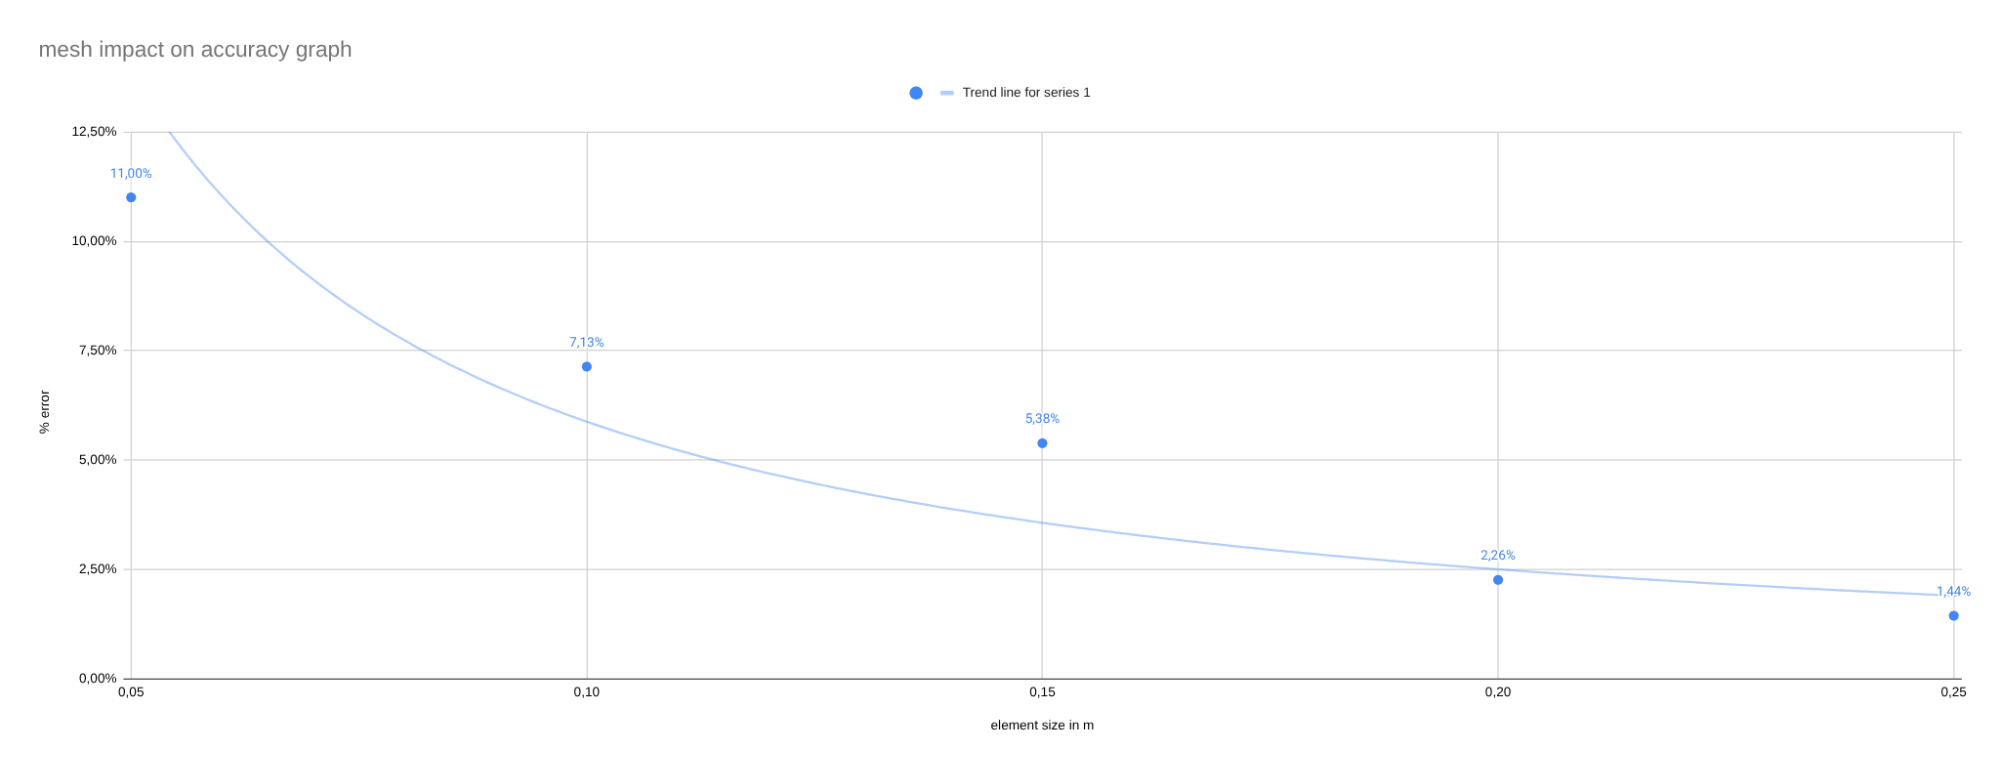
\includegraphics[width=0.8\textwidth]{image22.png}
\caption{Average \%error against element size of the mesh for the cube}
\label{fig:cube_mesh_error}
\end{figure}

This graph agin is for the cube and it is from the table above, i have taken the average \% error found at every mesh size and compared it too the mesh size.

I find this graph very useful for one specific object, but hardly useful for future comparisons or predictions, eventhough it shows the clear trend to more accurate measurements if the mesh density increases. Instead i have chosen to use this graph

\begin{table}[H]
\centering
\begin{tabular}{|c|c|}
\hline
\textbf{Amount of mesh elements} & \textbf{\% error} \\
\hline
52168 & 11.00\% \\
\hline
68605 & 7.13\% \\
\hline
97258 & 5.38\% \\
\hline
153590 & 2.26\% \\
\hline
341044 & 1.44\% \\
\hline
\end{tabular}
\end{table}

\begin{figure}[H]
\centering
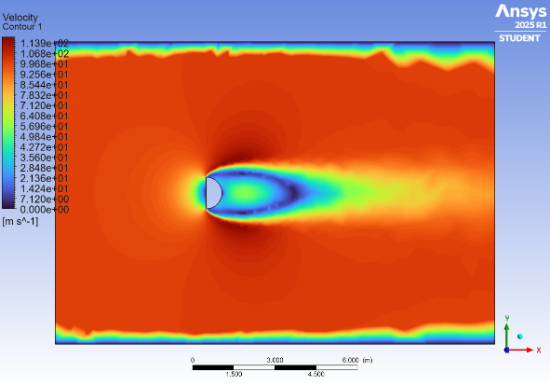
\includegraphics[width=0.8\textwidth]{image14.png}
\caption{Average \%error against amount of mesh elements for the cube}
\label{fig:cube_elements_error}
\end{figure}

I find this graph more useful, but because it shows the actual amount of elements, and as i said before these do varie across the different geometries, it will ease comparisons.

\begin{figure}[H]
    \centering
    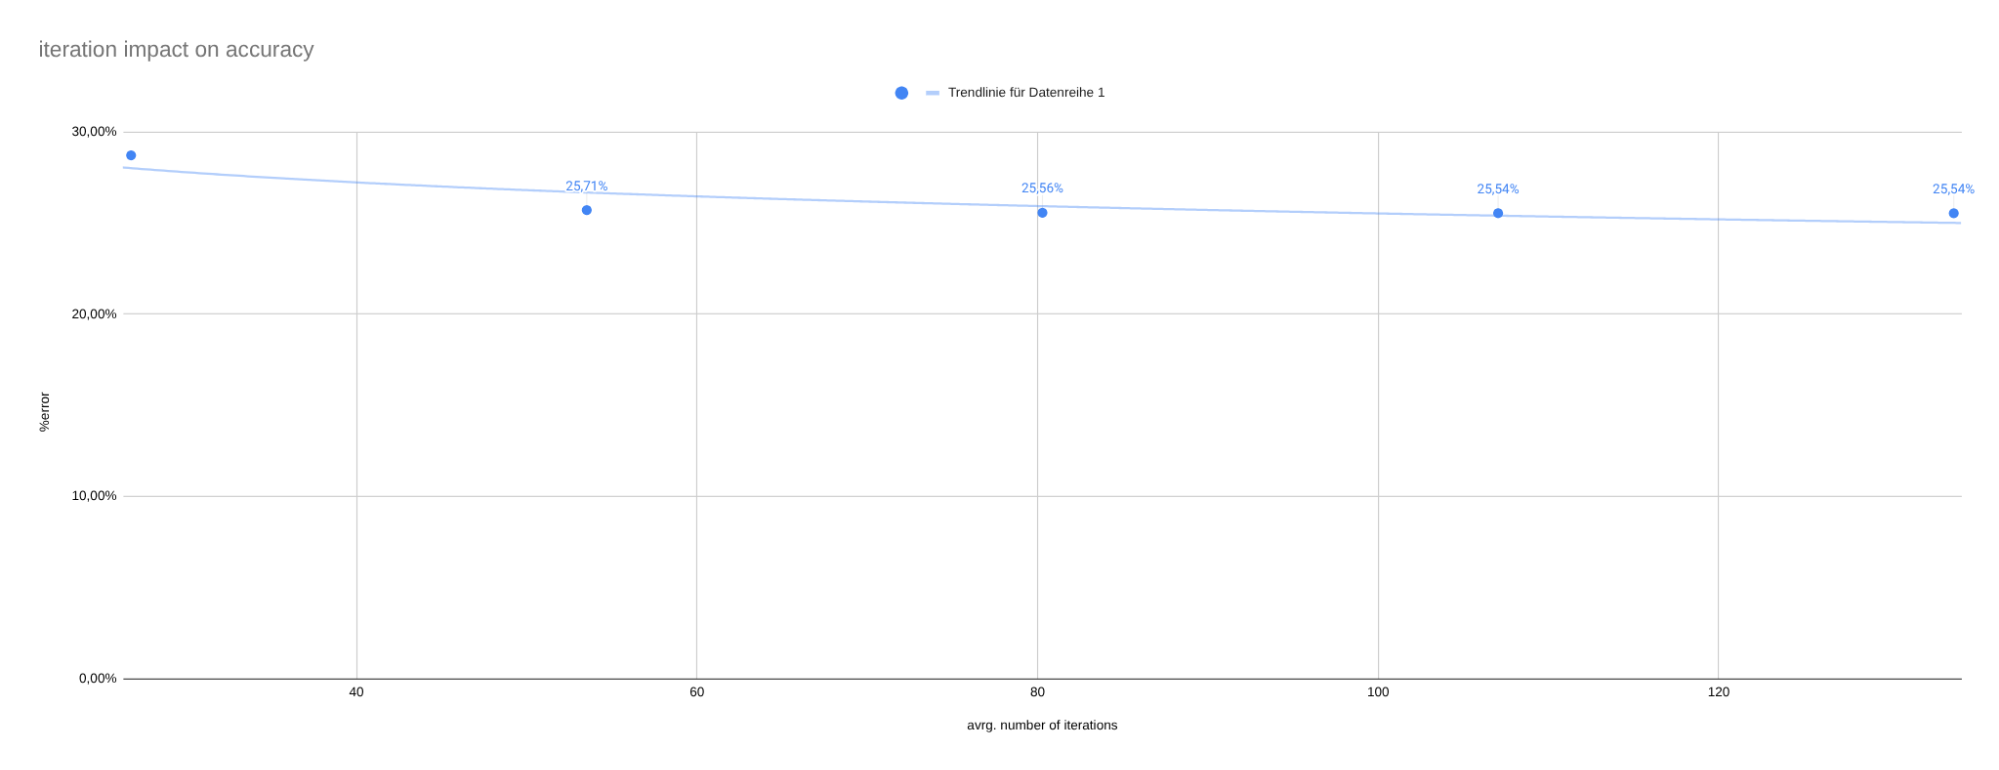
\includegraphics[width=0.8\textwidth]{image5.png}
    \caption{Average percentage error against fractional iterations for cube}
    \label{fig:cube_iterations_error}
\end{figure}

Figure \ref{fig:cube_iterations_error} shows clear correlation where increased iteration fraction reduces percentage error. Error decreases most at the start, making later changes harder to visualize.

\subsection{Results for Other Geometries}

\subsubsection{Cone Results}

\begin{table}[H]
\centering
\caption{Complete data collected for cone simulation}
\label{tab:cone_results}
\resizebox{\textwidth}{!}{%
\begin{tabular}{|c|c|c|c|c|c|c|c|c|c|c|c|}
\hline
\rowcolor{lightblue}
\textbf{Iteration} & \textbf{Expected (N)} & \textbf{Mesh 1 (N)} & \textbf{\% error} & \textbf{Mesh 2 (N)} & \textbf{\% error} & \textbf{Mesh 3 (N)} & \textbf{\% error} & \textbf{Mesh 4 (N)} & \textbf{\% error} & \textbf{Mesh 5 (N)} & \textbf{\% error} \\
\hline
1/5 of total & 3.06E+03 & 3.98E+03 & -30.01\% & 3.98E+03 & -30.05\% & 3.96E+03 & -29.26\% & 4.05E+03 & -32.39\% & 3.73E+03 & -21.86\% \\
\hline
2/5 of total & 3.06E+03 & 3.92E+03 & -27.99\% & 3.92E+03 & -27.91\% & 3.92E+03 & -27.99\% & 3.86E+03 & -25.90\% & 3.64E+03 & -18.76\% \\
\hline
3/5 of total & 3.06E+03 & 3.92E+03 & -27.93\% & 3.92E+03 & -27.87\% & 3.92E+03 & -28.00\% & 3.85E+03 & -25.63\% & 3.63E+03 & -18.39\% \\
\hline
4/5 of total & 3.06E+03 & 3.92E+03 & -27.92\% & 3.92E+03 & -27.85\% & 3.92E+03 & -28.00\% & 3.85E+03 & -25.59\% & 3.62E+03 & -18.34\% \\
\hline
5/5 of total & 3.06E+03 & 3.92E+03 & -27.91\% & 3.92E+03 & -27.85\% & 3.92E+03 & -28.00\% & 3.85E+03 & -25.59\% & 3.62E+03 & -18.34\% \\
\hline
\end{tabular}
}
\end{table}

\subsubsection{Half Sphere Results}

\begin{table}[H]
\centering
\caption{Complete data collected for half sphere simulation}
\label{tab:half_sphere_results}
\resizebox{\textwidth}{!}{%
\begin{tabular}{|c|c|c|c|c|c|c|c|c|c|c|c|}
\hline
\rowcolor{lightblue}
\textbf{Iteration} & \textbf{Expected (N)} & \textbf{Mesh 1 (N)} & \textbf{\% error} & \textbf{Mesh 2 (N)} & \textbf{\% error} & \textbf{Mesh 3 (N)} & \textbf{\% error} & \textbf{Mesh 4 (N)} & \textbf{\% error} & \textbf{Mesh 5 (N)} & \textbf{\% error} \\
\hline
1/5 of total & 7.17E+03 & 7.44E+03 & -3.84\% & 8.06E+03 & -12.43\% & 8.27E+03 & -15.42\% & 7.40E+03 & -3.26\% & 7.37E+03 & -2.91\% \\
\hline
2/5 of total & 7.17E+03 & 7.44E+03 & -3.85\% & 7.31E+03 & -1.98\% & 7.52E+03 & -4.94\% & 7.40E+03 & -3.32\% & 7.32E+03 & -2.14\% \\
\hline
3/5 of total & 7.17E+03 & 7.44E+03 & -3.84\% & 7.27E+03 & -1.50\% & 7.50E+03 & -4.71\% & 7.40E+03 & -3.32\% & 7.32E+03 & -2.08\% \\
\hline
4/5 of total & 7.17E+03 & 7.44E+03 & -3.84\% & 7.28E+03 & -1.55\% & 7.50E+03 & -4.70\% & 7.40E+03 & -3.31\% & 7.31E+03 & -2.06\% \\
\hline
5/5 of total & 7.17E+03 & 7.44E+03 & -3.85\% & 7.28E+03 & -1.53\% & 7.50E+03 & -4.70\% & 7.40E+03 & -3.29\% & 7.31E+03 & -2.06\% \\
\hline
\end{tabular}
}
\end{table}

\subsubsection{Streamline Body Results}

\begin{table}[H]
\centering
\caption{Complete data collected for streamline body simulation}
\label{tab:streamline_results}
\resizebox{\textwidth}{!}{%
\begin{tabular}{|c|c|c|c|c|c|c|c|c|c|c|c|}
\hline
\rowcolor{lightblue}
\textbf{Iteration} & \textbf{Expected (N)} & \textbf{Mesh 1 (N)} & \textbf{\% error} & \textbf{Mesh 2 (N)} & \textbf{\% error} & \textbf{Mesh 3 (N)} & \textbf{\% error} & \textbf{Mesh 4 (N)} & \textbf{\% error} & \textbf{Mesh 5 (N)} & \textbf{\% error} \\
\hline
1/5 of total & 2.45E+02 & 2.54E+02 & -3.51\% & 2.52E+02 & -2.77\% & 2.40E+02 & 2.04\% & 2.25E+02 & 8.16\% & 2.00E+02 & 18.44\% \\
\hline
2/5 of total & 2.45E+02 & 2.53E+02 & -3.40\% & 2.52E+02 & -2.73\% & 2.40E+02 & 1.93\% & 2.25E+02 & 8.05\% & 2.00E+02 & 18.56\% \\
\hline
3/5 of total & 2.45E+02 & 2.53E+02 & -3.45\% & 2.52E+02 & -2.79\% & 2.40E+02 & 2.02\% & 2.25E+02 & 8.10\% & 1.99E+02 & 18.58\% \\
\hline
4/5 of total & 2.45E+02 & 2.53E+02 & -3.40\% & 2.52E+02 & -2.83\% & 2.40E+02 & 1.88\% & 2.25E+02 & 8.11\% & 1.99E+02 & 18.60\% \\
\hline
5/5 of total & 2.45E+02 & 2.53E+02 & -3.45\% & 2.52E+02 & -2.81\% & 2.40E+02 & 1.86\% & 2.25E+02 & 8.11\% & 1.99E+02 & 18.59\% \\
\hline
\end{tabular}
}
\end{table}

\subsubsection{Long Cylinder Results}

\begin{table}[H]
\centering
\caption{Complete data collected for long cylinder simulation}
\label{tab:cylinder_results}
\resizebox{\textwidth}{!}{%
\begin{tabular}{|c|c|c|c|c|c|c|c|c|c|c|c|}
\hline
\rowcolor{lightblue}
\textbf{Iteration} & \textbf{Expected (N)} & \textbf{Mesh 1 (N)} & \textbf{\% error} & \textbf{Mesh 2 (N)} & \textbf{\% error} & \textbf{Mesh 3 (N)} & \textbf{\% error} & \textbf{Mesh 4 (N)} & \textbf{\% error} & \textbf{Mesh 5 (N)} & \textbf{\% error} \\
\hline
1/5 of total & 5.02E+03 & 5.12E+03 & -1.85\% & 5.17E+03 & -2.94\% & 5.01E+03 & 0.24\% & 5.28E+03 & -5.16\% & 5.28E+03 & -5.14\% \\
\hline
2/5 of total & 5.02E+03 & 5.11E+03 & -1.79\% & 5.19E+03 & -3.29\% & 5.02E+03 & 0.04\% & 5.28E+03 & -5.17\% & 5.28E+03 & -5.12\% \\
\hline
3/5 of total & 5.02E+03 & 5.14E+03 & -2.33\% & 5.19E+03 & -3.34\% & 5.04E+03 & -0.32\% & 5.28E+03 & -5.14\% & 5.28E+03 & -5.13\% \\
\hline
4/5 of total & 5.02E+03 & 5.13E+03 & -2.24\% & 5.19E+03 & -3.29\% & 5.04E+03 & -0.34\% & 5.28E+03 & -5.18\% & 5.28E+03 & -5.13\% \\
\hline
5/5 of total & 5.02E+03 & 5.12E+03 & -1.98\% & 5.19E+03 & -3.33\% & 5.04E+03 & -0.31\% & 5.28E+03 & -5.16\% & 5.28E+03 & -5.13\% \\
\hline
\end{tabular}
}
\end{table}

Some investigated objects showed outliers where simulated results became more accurate with fewer iterations or decreasing mesh density. These are considered outliers because simulations continue until reaching most accurate results (the basis of residuals). When less dense meshes created more accurate results, this was likely caused by complex geometry modeling difficulties and insufficient boundary conditions. These outliers are excluded from final results.

\subsection{Overall Results Summary}

\begin{table}[H]
\centering
\caption{Summary of average iterations and mesh elements with corresponding errors across all simulations}
\label{tab:overall_summary}
\begin{tabular}{|c|c|c|c|c|c|}
\hline
\rowcolor{lightblue}
\textbf{Avg Iterations} & \textbf{\% Error} & & \textbf{Mesh Elements} & \textbf{\% Error} & \textbf{Time/Iteration (s)} \\
\hline
77 & 14.29\% & & 114,025 & 14.40\% & 14 \\
\hline
154 & 11.42\% & & 119,628 & 13.08\% & 14.5 \\
\hline
231 & 11.26\% & & 133,739 & 13.51\% & 14 \\
\hline
308 & 11.24\% & & 171,610 & 10.86\% & 15 \\
\hline
385 & 11.24\% & & 308,837 & 7.61\% & 28.5 \\
\hline
\end{tabular}
\end{table}

Average time per iteration was recorded because reading total time would be extremely difficult. Time per iteration correlates with mesh density, showing higher mesh density requires longer simulation time. Although generally the final iterations take less time and iterations don't all require equal time, averages were used without decimal precision since millisecond variations could be random and noisy.

\begin{figure}[H]
    \centering
    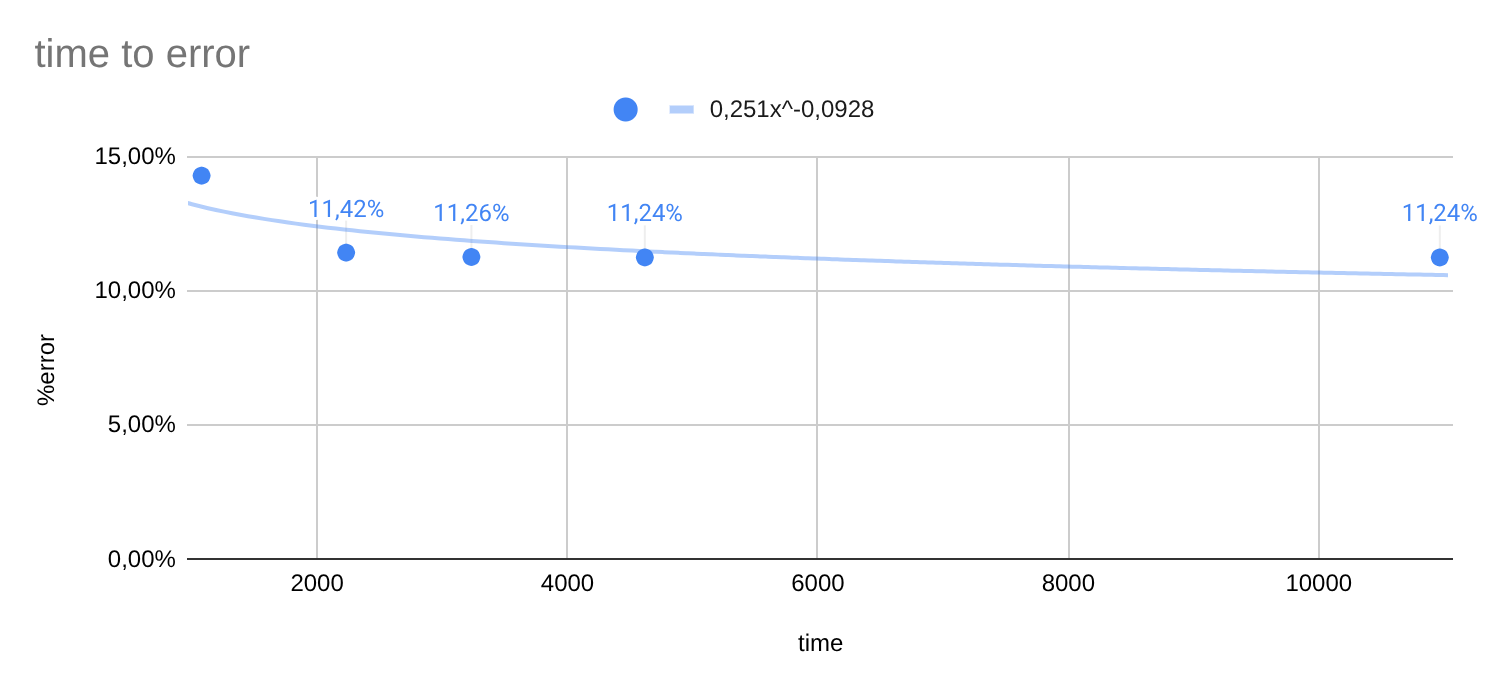
\includegraphics[width=0.8\textwidth]{image6.png}
    \caption{Time versus average percentage error across all geometries}
    \label{fig:time_vs_error}
\end{figure}

When looking at the final results it is very clear that the simulations go on for a very long time, even if not allot of accuracy is gained, the function of increasing accuracy is assemptoting somewhere to 11 \%, and especially after the 3 hour mark not allot of accuracy is gained and allot of valuable energy is waisted. So considering that my experimental values where only to 3 significant figures i have stated that a change in less than 0.02\% is not worth the time as it is insignificant to 3 significant figures, as a result instead of investing more than 10000 seconds on average for a simulaton only 4592 seconds would arguable give good enough results, this would more than half the time and save so much energy, if i go back reducing the accuracy for both variables by 0.01\% this means only 264 iterations on average is how long a simulation should run.

\begin{figure}[H]
\centering
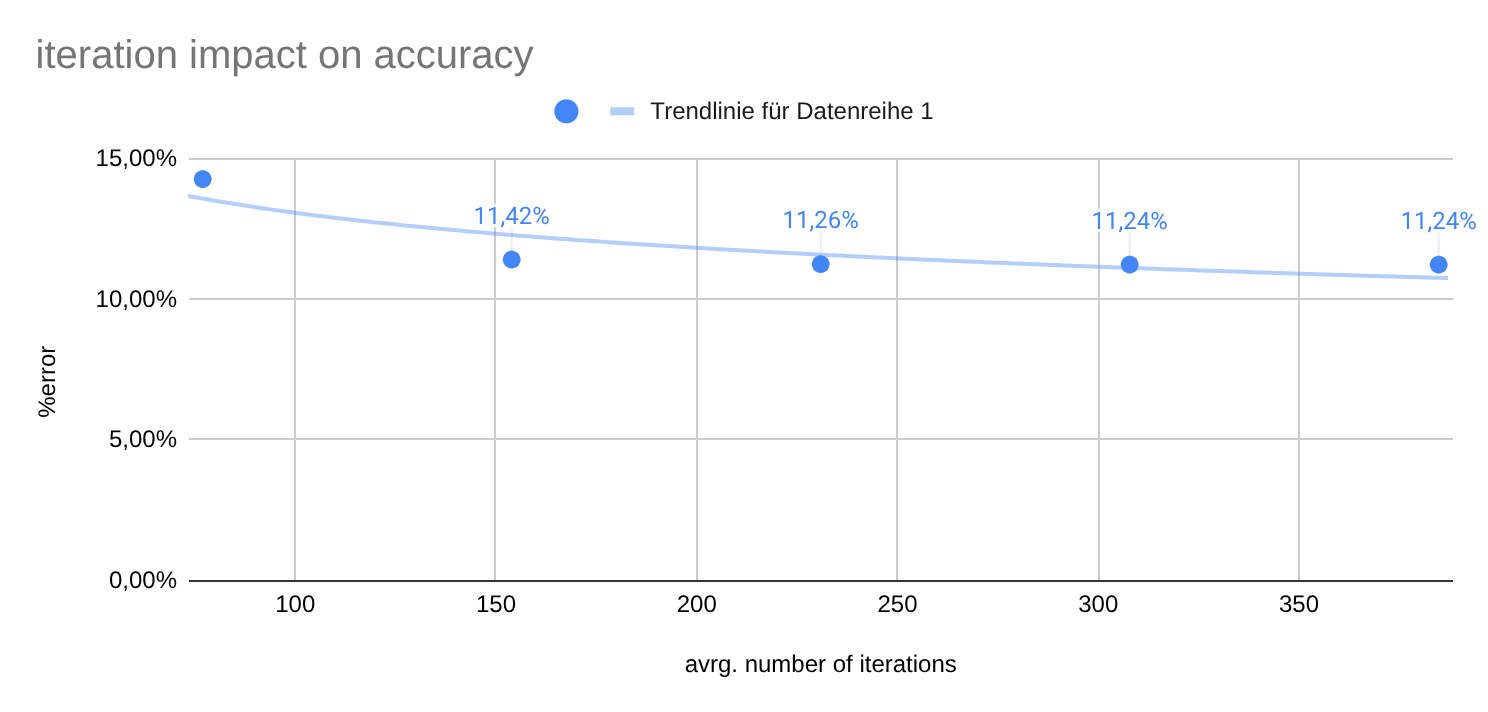
\includegraphics[width=0.8\textwidth]{image11.png}
\caption{Average amount of total iterations against average \% error}
\label{fig:iterations_final}
\end{figure}

whilst i found that 30234 mesh elements are sufficient for a volume of 1936m3.

\begin{figure}[H]
\centering
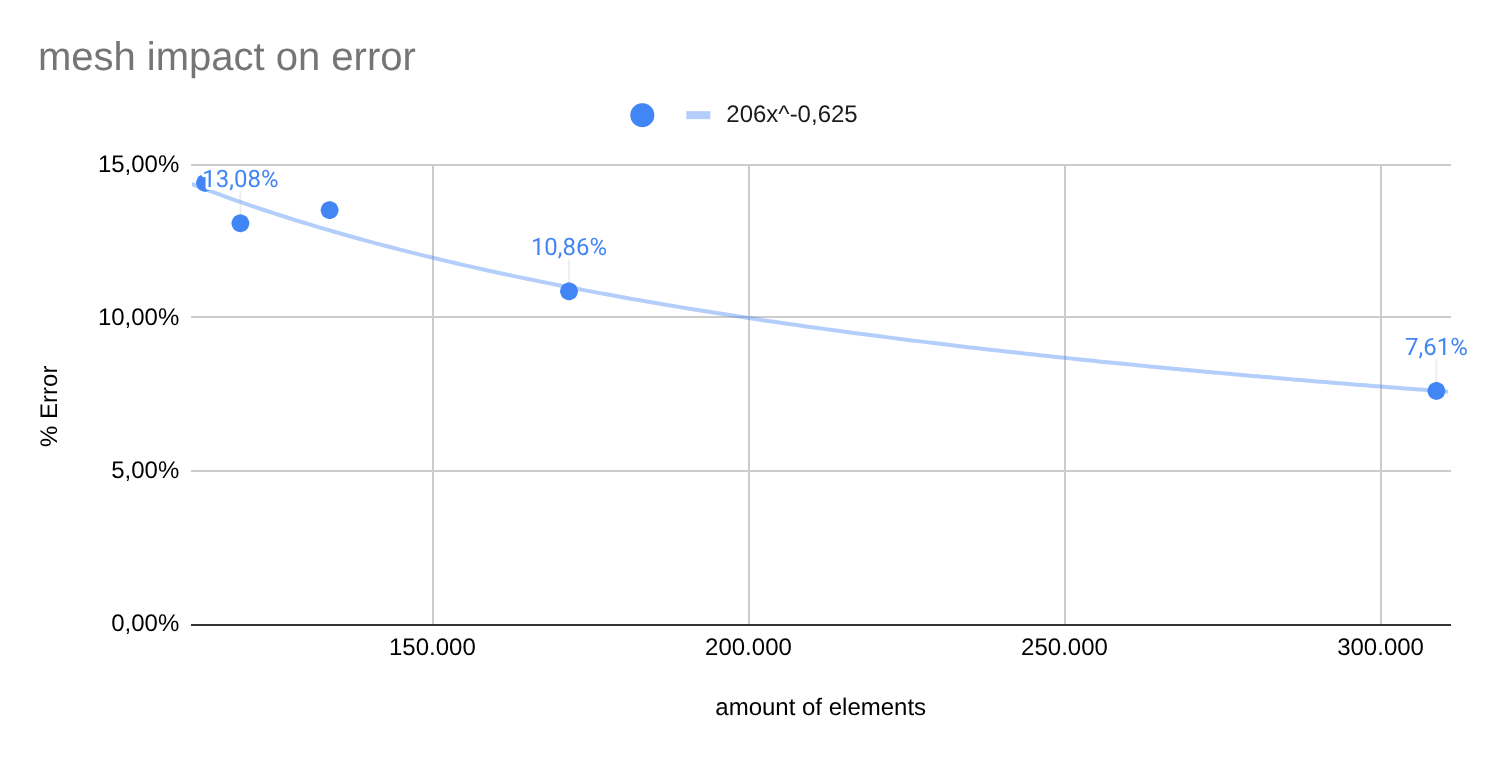
\includegraphics[width=0.8\textwidth]{image2.png}
\caption{Average amount of mesh elements against average \% error}
\label{fig:mesh_final}
\end{figure}

\subsection{Comparison with IB Fluid Drag Formula}

To see if both parts of the assumption we have in ib have a impact on the simulations i have simulated a cube using a laminar flow model, in this case i am only exploring complex objects. 

\begin{table}[H]
\centering
\caption{Further studies data for a cube assuming laminar flow}
\label{tab:laminar_cube}
\begin{tabular}{|c|c|c|c|}
\hline
\textbf{Iteration} & \textbf{Expected /N} & \textbf{simulation} & \textbf{\% error} \\
\hline
1/5 of total & 6.43E+03 & 7.30E+03 & -13.50\% \\
\hline
2/5 of total & 6.43E+03 & 6.90E+03 & -7.25\% \\
\hline
3/5 of total & 6.43E+03 & 7.39E+03 & -14.91\% \\
\hline
4/5 of total & 6.43E+03 & 6.83E+03 & -6.24\% \\
\hline
5/5 of total & 6.43E+03 & 7.29E+03 & -13.35\% \\
\hline
\end{tabular}
\end{table}

actual the simulations results are not as far of as i thought they might be, the laminar flow model is not as good as the k.epsilon and the readings were variating alot, nevertheless i think the difference is not to far off, because the flow was nto as turbulent to start off with. All simulations were done at the highest mesh density explored.

\begin{table}[H]
\centering
\caption{Further studies data for a sphere assuming nothing}
\label{tab:sphere_ib}
\begin{tabular}{|c|c|c|c|c|}
\hline
\textbf{Iteration} & \textbf{Expected /N} & \textbf{IB Expected /N} & \textbf{simulation} & \textbf{\% error} \\
\hline
1/5 of total & 2.88E+03 & 1.92E-02 & 2.84E+03 & 1.43\% \\
\hline
2/5 of total & 2.88E+03 & 1.92E-02 & 2.85E+03 & 1.08\% \\
\hline
3/5 of total & 2.88E+03 & 1.92E-02 & 2.85E+03 & 1.05\% \\
\hline
4/5 of total & 2.88E+03 & 1.92E-02 & 2.85E+03 & 0.96\% \\
\hline
5/5 of total & 2.88E+03 & 1.92E-02 & 2.85E+03 & 0.98\% \\
\hline
\end{tabular}
\end{table}

Here i am comparing how big the influence of turbulent flow is one the assumption, in this case i should be able to use the ib formula, aswell because the object used is a sphere, my simulation of course was not far off the expectation. I would not have to simulate it probably and i could have compared the different equations bythemself, as we can see the ib formula and the actual values are really far of, i think turbulence is one of the reasons this is happening, but i think the big difference in the forces is due to the fact that the ib formula is not considering that force increases squard to the velocity, and this is at 100 ms$^{-1}$

\section{Conclusion}

After finishing all tables this are the average iterations and the average mesh with their according average \%error across all simulations,

\begin{table}[H]
\centering
\caption{All average \% iteration against all \% error and all average mesh elements against average \% error}
\label{tab:final_summary}
\begin{tabular}{|c|c|c|c|c|c|}
\hline
\textbf{Average amount of iteration} & \textbf{\% error} &  & \textbf{Amount of mesh elements} & \textbf{\%error} & \textbf{time/ iteration} \\
\hline
77 & 14.29\% &  & 114.025 & 14.40\% & 14 \\
\hline
154 & 11.42\% &  & 119.628 & 13.08\% & 14.5 \\
\hline
231 & 11.26\% &  & 133.739 & 13.51\% & 14 \\
\hline
308 & 11.24\% &  & 171.610 & 10.86\% & 15 \\
\hline
385 & 11.24\% &  & 308.837 & 7.61\% & 28.5 \\
\hline
\end{tabular}
\end{table}

Throughout the recording of the results i also recorder the average time it took to take to simulate one iteration, i used averages, because reading the total time would have been extremely hard. I compared them to mesh density 
Just adding the time per iteration on the right. This shows a correlation, where higher mesh density means longer time to simulate.
And because it is time per iteration, this means that time per iteration is directly related, even though i have to say that generally the last few iterations take less time and not every iterations takes the same amount of time, that is why i used averages and i went to no decimal place in my recordings, because variation in the milliseconds could be random and noisy.

\begin{figure}[H]
\centering
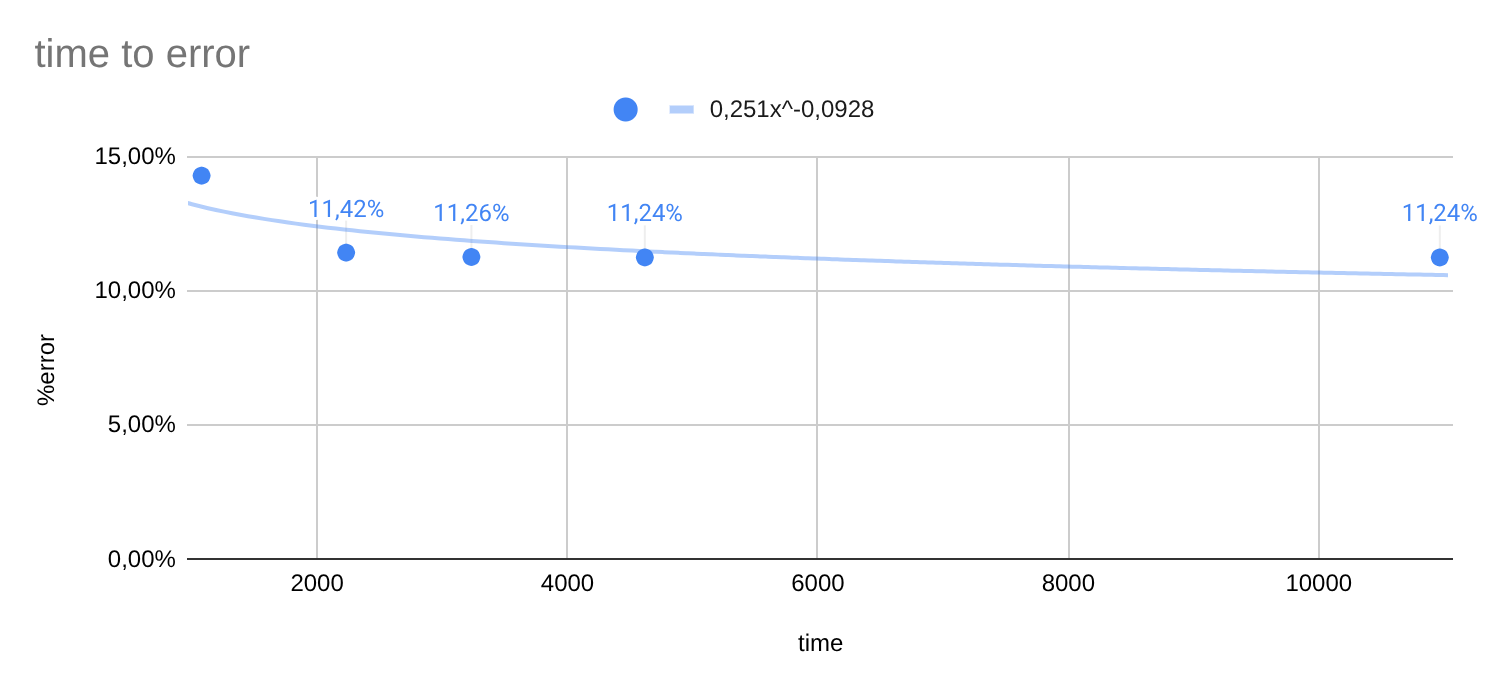
\includegraphics[width=0.8\textwidth]{image6.png}
\caption{Across all geometries, time against average\% error}
\label{fig:time_vs_error}
\end{figure}

I have realized when analysing my findings that two of the investigated objects show outliers, where the simulated number gets more accurate with less iterations or with decreasing mesh density, i think i can rightfully say that they are outliers, because the simulation will carry on until the simulation thinks it has reached the most accurate result, this is the base idea of the residuals. And when the less dense mesh created more accurate results this was also a outlier as this was most probably caused, because the geometry was very complex to model for me and there were not allot of boundaries given. I have excluded these from my final results as a result.
    \item K-epsilon turbulence modeling provides substantially better accuracy than laminar assumptions for complex geometries
    \item Computational resources can be optimized without sacrificing engineering-relevant accuracy
\end{itemize}

This research provides valuable insights for engineers and researchers seeking to optimize CFD simulation parameters, ultimately contributing to more sustainable computational practices in fluid dynamics analysis.

\section{Improvements}

I have tried to apply my findings on real world use cases, i tried to simulate the drag experienced by a tesla modes s plaid as it had a publicly known very low drag coefficient. Unfortunately my computer could not handle the complexity that a car has so i could not find if my results can be used in the real world, next time i would want to try out if it works for engineers aswell. 

Unfortunately some of the geometries which i had experimental data to test against were described very badly like a long cylinder and streamline body, next time i would try and get my own experimental data to be sure that both have the same boundary conditions.

\section{References}

- Citing academic papers, CFD textbooks, and engineering articles.

Assets:

\begin{figure}[H]
\centering
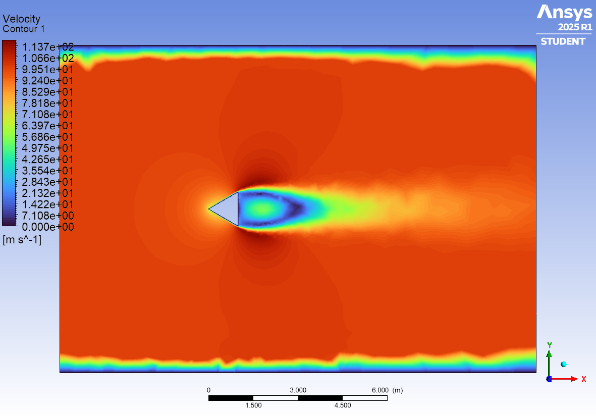
\includegraphics[width=0.8\textwidth]{image3.png}
\caption{Additional simulation visualization 1}
\label{fig:asset1}
\end{figure}

\begin{figure}[H]
\centering
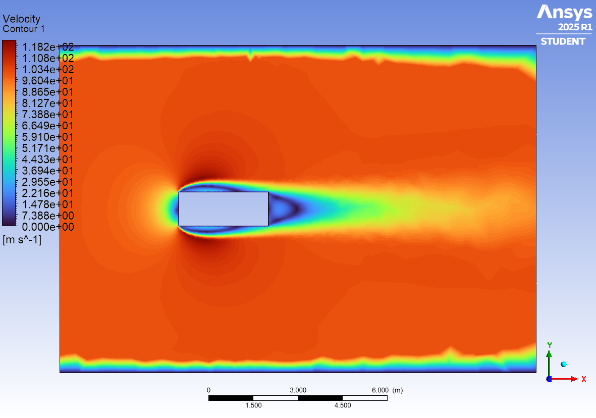
\includegraphics[width=0.8\textwidth]{image10.png}
\caption{Additional simulation visualization 2}
\label{fig:asset2}
\end{figure}

\begin{figure}[H]
\centering
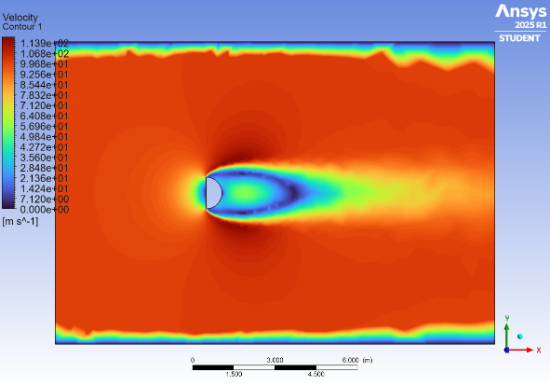
\includegraphics[width=0.8\textwidth]{image16.png}
\caption{Additional simulation visualization 3}
\label{fig:asset3}
\end{figure}

\begin{figure}[H]
\centering
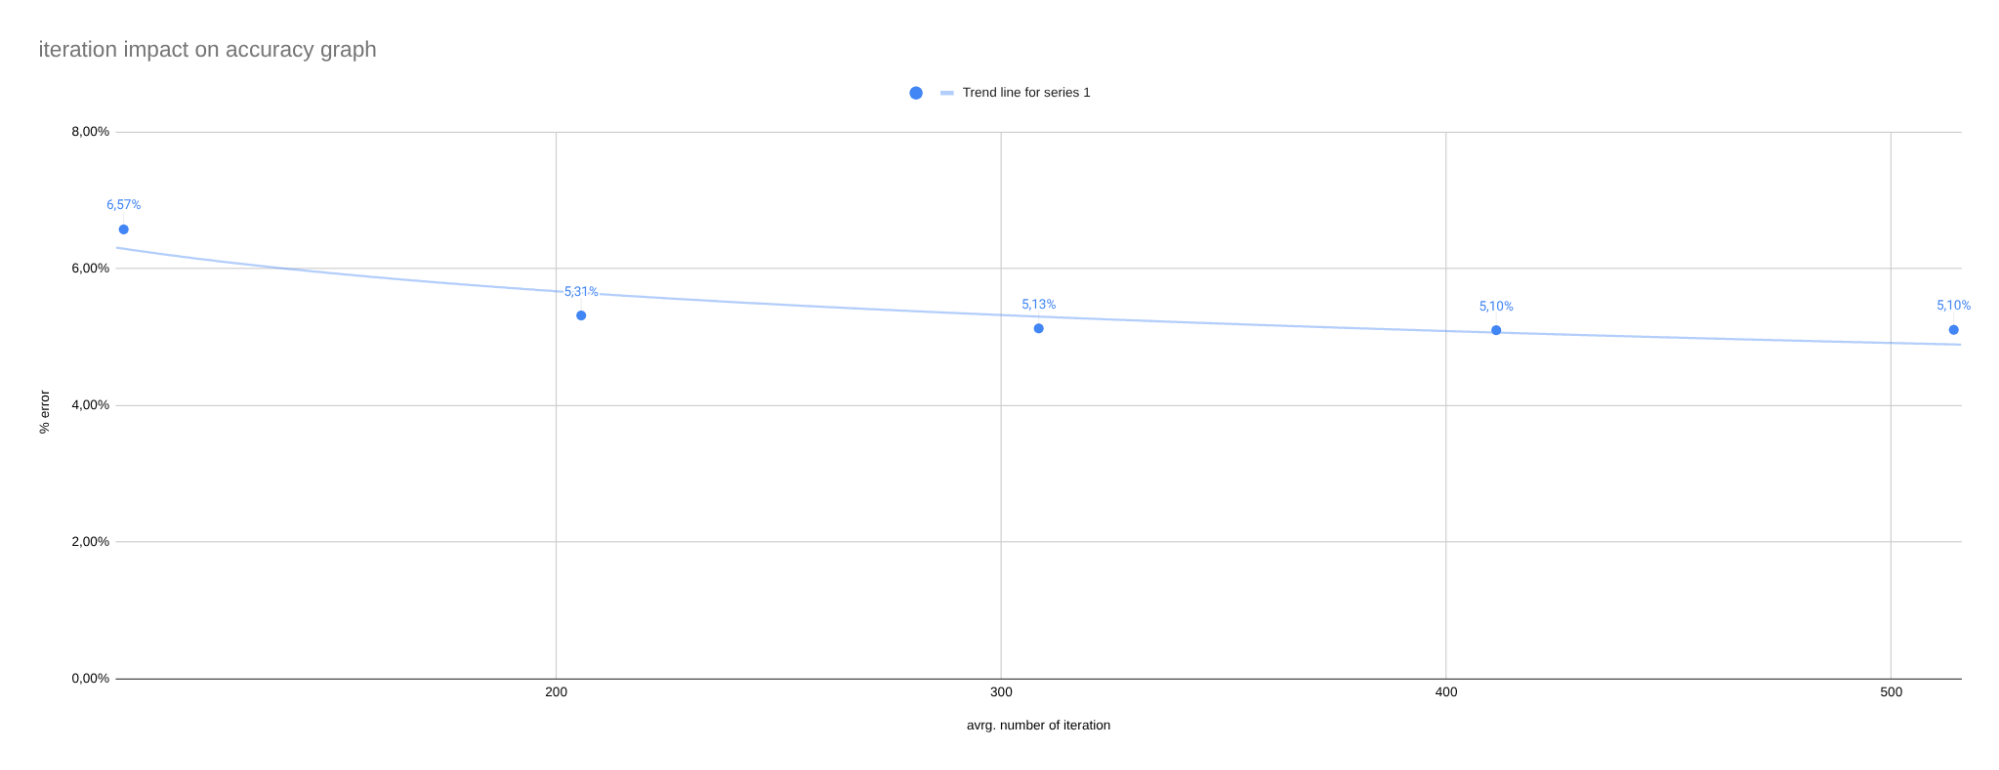
\includegraphics[width=0.8\textwidth]{image13.png}
\caption{Extra pictures depicting that i actually did the simulations}
\label{fig:asset4}
\end{figure}

\end{document}
